\section{Numerical Methods}\label{Section:Numerics}
Because \cref{Eqn:HEMBasic} has no closed form solution as presented, numerical approximations are needed to observe the theoretical evolution of the system.
First, a number of spatial discretizations will be discussed such that the system can be put into a so-called semi-discrete form.
Then, time integration methods will be discussed.

\subsection{Spatial Discretization}\label{Subsection:SpatialDiscretization}
Before discussing the spatial discretizations, the end goals of the methods should be considered.
\Cref{Figure:ComputationGeometry} shows the computational geometry to ultimately studied.
Unlike a  majority of the literature, the novelty of this research aims to tackle the stability of a non-simple, closed curve.
Because the curve is non-simple, there are branch points which have more than one possible path, and the numerical methods must be amenable to this requirement.
Also, the tank (the large volume topping the model) is open to atmosphere that allows for an unrecoverable loss of mass to the atmosphere, so the method should be able to allow for a flow of liquid from the system to an infinite sink.

\begin{figure}%
    \centering
    \caption[Geomtry to model]{Geometry required to model.  
                The black, directed line is the non-simple, closed curve along which the conservation laws must be satisfied.
                 The blue and red outlines denote the cooling and heating zones, respectively.}%
    \label{Figure:ComputationGeometry}%
    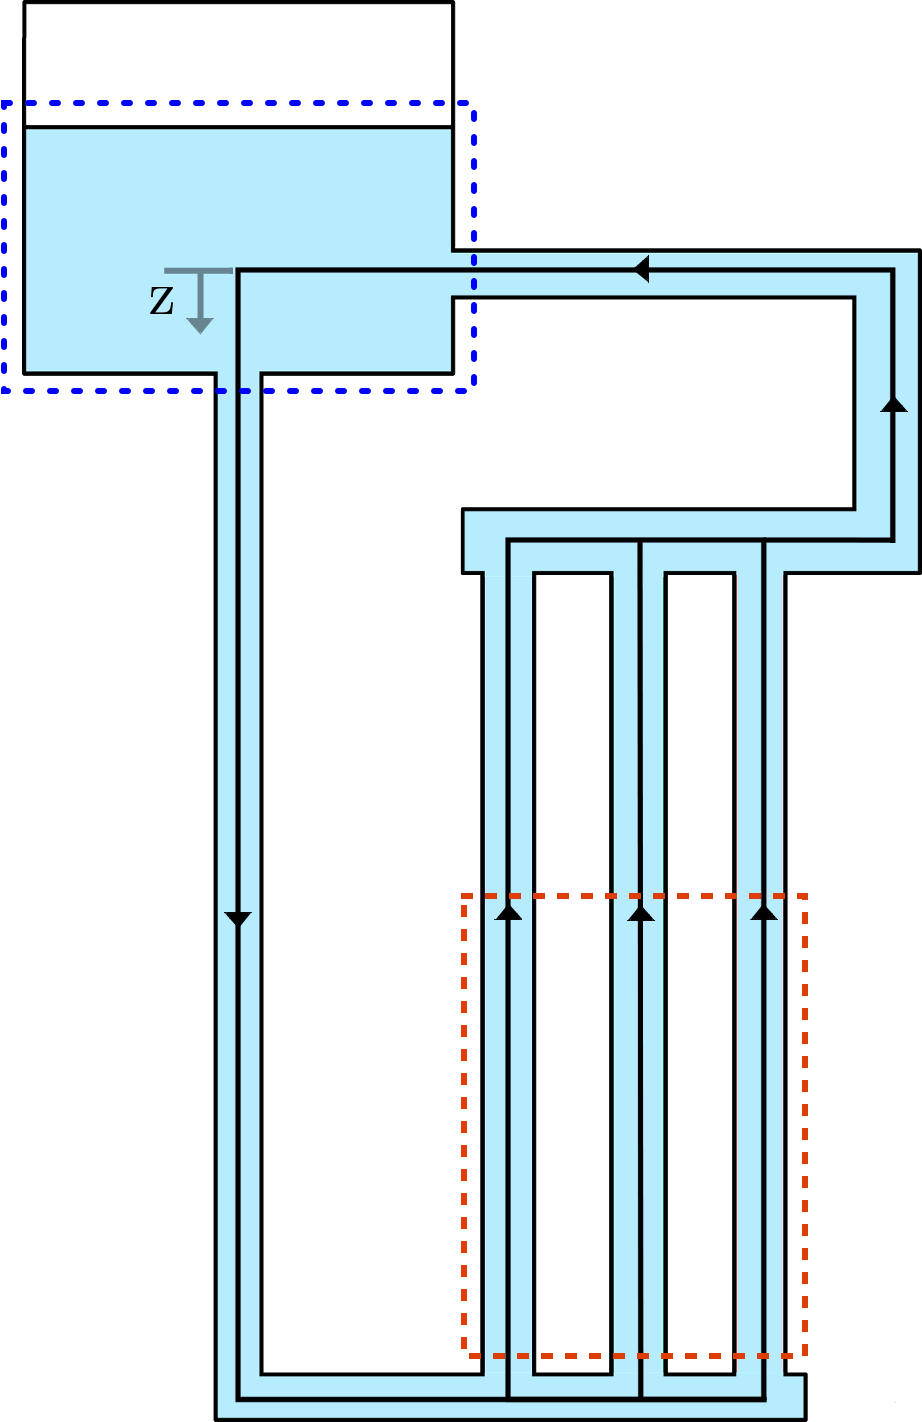
\includegraphics[height=3.5in]{ComputationalGeometry}%
\end{figure}


\subsubsection{Collocated Nodal (Steady-state only)}\label{Subsubsection:CollocatedNodal}
The simplest (yet hardest) numerical example to begin with is the steady-state nodal method for a simply closed loop.
Setting the time derivative of \cref{Eqn:HEMBasic} to $0$ yields 
\begin{equation}
    \pdiff{}{z}\begin{bmatrix}
                    \rhou                 \\
                    u\,\rhou + P(\rho,i)   \\
                    u\left[\rhoi  + P(\rho,i)\right]
                \end{bmatrix}
             =  
    \begin{bmatrix}
        0 \\% \mdotloss                \\
        \rho{g(z)} - \frac{\Keff(\qCon)}{2} u\,|\rhou|  \\
        \dot{Q}\subs{add}(z,t)
    \end{bmatrix}
    \label{Eqn:HEMBasicSS}
\end{equation}
and now, for ease of discussion and writing, the individual flux and source functions will be numbered:
\begin{align}
    \FluxFun{\qCon;x} &=    
                \begin{bmatrix}
                    F^1(\qCon;\Space)\\
                    F^2(\qCon;\Space)\\
                    F^3(\qCon;\Space)\\
                \end{bmatrix}
           =    \begin{bmatrix}
                    \rhou                 \\
                    u\,\rhou + P(\rho,i)   \\
                    u\left[\rhoi  + P(\rho,i)\right]
                \end{bmatrix} \\
    \SourceFun{\qCon,\Space} &=  
            \begin{bmatrix}
                    S^1(\qCon,\Space)\\
                    S^2(\qCon,\Space)\\
                    S^3(\qCon,\Space)\\
                \end{bmatrix}
             =  \begin{bmatrix}
                    0 \\% \mdotloss                \\
                    \rho{g(z)} - \frac{\Keff(\qCon)}{2} u\,|\rhou|  \\
                    \dot{Q}\subs{add}(\Space,t)
                \end{bmatrix},
\end{align}

Due to the nonlinearity of the problem, a numerical approximation to the solution of \cref{Eqn:HEMBasicSS} will be attempted.
Let $\Space^\dagger$ be a discrete partitioning of $\Space$ into of the form
\[
    \Space_g = \Space_1 < \Space_2 < \Space_3 < ... < \Space_N < \Space_{N+1} = \Space_g,
\]
where $N$ is the number of approximate states.
It is important to notice that since $\Space$, and therefore $\Space^\dagger$, is a closed circuit, $\Space_1$ and $\Space_{N+1}$ map to the same location $\Space_g$.
Integrating \cref{Eqn:HEMBasicSS} over a given partition of $\Space^\dagger$, to be called a control volume, yields
\begin{equation}
    \Flux(\qCon;\Space_{i+1}) - \Flux(\qCon;\Space_i) = \Weight_i \Source(\qCon,\Space_{i}) + \Weight_{i+1} \Source(\qCon,\Space_{i+1}) + \mathcal{O}(|\Space_{i+1}-\Space_i|^2),
    \label{Eqn:IntegrationTrueSolution}
\end{equation}
where the source function has been integrated via the trapezoidal rule to yield a second order approximation to the system.
While the true solution \qCon exactly balances \cref{Eqn:IntegrationTrueSolution}, if a discrete approximation $\qCon^\dagger$ is introduced and the trapezoidal error term ignored, the balance will more than likely be lost.  This loss of balance results in a residual (error) function defined by
\begin{equation}
    \Rez_i(\qCon^\dagger) = \left[\Flux(\qCon^\dagger;\Space_{i+1}) - \Flux(\qCon^\dagger;\Space_i)\right] -
                       \left[\Weight_i \Source(\qCon^\dagger;\Space_{i}) + \Weight_{i+1} \Source(\qCon^\dagger;\Space_{i+1})\right].
    \label{Eqn:IntegrationApproxSolution}
\end{equation}
This equation leads to a system of nonlinear equations in $\qCon^\dagger$:
\begin{equation}
\begin{split}
    \Rez_1(\qCon^\dagger)     &= 
            \left[\Flux(\qCon^\dagger;\Space_{2}) - \Flux(\qCon^\dagger;x_1)                               \right] -
            \left[\Weight_1 \Source(\qCon^\dagger;\Space_{1}) + \Weight_{2  } \Source(\qCon^\dagger;\Space_{2  }) \right] \\[0.1em]
    \Rez_2(\qCon^\dagger)     &= \left[\Flux(\qCon^\dagger;\Space_{3}) - \Flux(\qCon^\dagger;x_2)                               \right] -
                              \left[\Weight_2 \Source(\qCon^\dagger;\Space_{2}) + \Weight_{3  } \Source(\qCon^\dagger;\Space_{3  }) \right] \\[0.0em]
                           &  \vdots                                                                                      \\
    \Rez_{N-1}(\qCon^\dagger) &= \left[\Flux(\qCon^\dagger;\Space_{N}) - \Flux(\qCon^\dagger;\Space_{N-1})                           \right] -
                              \left[\Weight_N \Source(\qCon^\dagger;\Space_{N}) + \Weight_{N-1} \Source(\qCon^\dagger;\Space_{N-1}) \right] \\[0.1em]
    \Rez_N(\qCon^\dagger)     &= \left[\Flux(\qCon^\dagger;\Space_{1}) - \Flux(\qCon^\dagger;\Space_N)                               \right] -
                              \left[\Weight_1 \Source(\qCon^\dagger;\Space_{1}) + \Weight_{N  } \Source(\qCon^\dagger;\Space_{N  }) \right].
\end{split}\label{Eqn:EachResidualEquation}
\end{equation}
If a $\qCon^\dagger$ is found at each location in $\Space^\dagger$ such that each of the residuals is approximately $0$, then $\qCon^\dagger$ is a solution to \cref{Eqn:IntegrationApproxSolution}.

\Cref{Eqn:EachResidualEquation} will now be written in a more succinct form to examine the structure of the system.
Letting $\Flux^\dagger$ be the discrete, ordered flux function defined by
\begin{equation}
    \Flux^\dagger = \Flux(\qCon^\dagger;\Space^\dagger) =
    \begin{bmatrix}
        [F^1(\qCon^\dagger;\Space_1)\,...\,F^1(\qCon^\dagger;\Space_N)]^T \\
        [F^2(\qCon^\dagger;\Space_1)\,...\,F^2(\qCon^\dagger;\Space_N)]^T \\
        [F^3(\qCon^\dagger;\Space_1)\,...\,F^3(\qCon^\dagger;\Space_N)]^T 
    \end{bmatrix}
\end{equation}
and $\Source^\dagger$ be the discrete, ordered source function defined by
\begin{equation}
    \Source^\dagger = \Source(\qCon^\dagger;\Space^\dagger) =
    \begin{bmatrix}
        [S^1(\qCon^\dagger,\Space_1)\,...\,S^1(\qCon^\dagger,\Space_N)]^T \\
        [S^2(\qCon^\dagger,\Space_1)\,...\,S^2(\qCon^\dagger,\Space_N)]^T \\
        [S^3(\qCon^\dagger,\Space_1)\,...\,S^3(\qCon^\dagger,\Space_N)]^T
    \end{bmatrix},
\end{equation}
\cref{Eqn:EachResidualEquation} can be rewritten as
\begin{equation}
    \Rez^\dagger = \mathbb{C}_F \Flux^\dagger - \mathbb{C}_S \Source^\dagger.
\end{equation}
The matrices $\mathbb{C}_F$ and $\mathbb{C}_S$ are the so-called system connectivity matrices as they describe how the individual control volumes  of the whole system are linked to one another.  Each of these connectivity matrices has the block structure
\begin{align}
    \mathbb{C}_* &=  \begin{bmatrix}
                        \mathbf{C}_* & \mathbf{0}   & \mathbf{0} \\
                        \mathbf{0}   & \mathbf{C}_* & \mathbf{0} \\
                        \mathbf{0}   & \mathbf{0}   & \mathbf{C}_* 
                     \end{bmatrix},
    \label{Eqn:SysConnMatrices}
\end{align}
where $\mathbf{C}_*$ are law connectivity matrices, as they describe how a given conservation law is discretely linked in the system.
The flux function's law connectivity matrix  is $N \times N$ and has the sparse form
\begin{align}
    \mathbf{C}_F &=  \begin{bmatrix}
                        -1     & +1  &        &        &          \\
                               & -1 & +1      &        &          \\
                               &    & \ddots & \ddots &          \\
                               &    &        &  -1    &  +1       \\
                        +1      &    &        &        & -1
                     \end{bmatrix}.
\end{align}
Similarly, the source function's law connectivity matrix has the sparse form
\begin{align}
    \mathbf{C}_S &=  \begin{bmatrix}
                       \Weight_1 & \Weight_2 &          &              &          \\
                                & \Weight_2 & \Weight_3 &              &          \\
                                &          & \ddots   & \ddots       &          \\
                                &          &          & \Weight_{N-1} & \Weight_N \\
                       \Weight_1 &          &          &              & \Weight_N
                     \end{bmatrix}.
\end{align}
It is noted that these submatrices are singular, due to a doubly reflective boundary conditions.
That being the case, a solution not involving inversion of the matrices will be presented in \cref{Section:SSSolver}.


\subsubsection{Staggered Finite Volume}
A problem with the previous section is not only the singularness of the connectivity matrices, but also that the method does not lend itself to arbitrary two-dimensional geometry per the problem to be investigated.
Therefore, it is natural to switch over to a finite volume method that uses time integration to find possible steady-states.
It will be noted that this section's title emphasizes ``staggered'' since there are collocated finite volume emthods.
However, collocated schemes were not investigated here because it is very hard for them to properly conserve certain variables exactly \cite{morinishi_fully_1998}.

A staggered mesh involves integrating the conservation laws over two different domains: control volumes and momentum cells.
The control volumes typically hold all scalar quantities while the momentum cells serve as information propagators for the system with limited fluid residence time.
Also, it is valuable to integrate the equations in three dimensions such that the gradients explicitly become surface integrals.
Therefore, the equation's original form (\cref{Eqn:HEMBasic}) will be written with multidimensional derivatives (though this will be temporary and the flows are still, technically, one-dimensional).

Integrating the conservation of mass and energy equations over a closed, fixed volume \CVvol yields
\begin{equation}
    \iiint_{\CVvol}\pdiff{}{t}\begin{bmatrix}
                   \rho \\
                   \rhoi 
                \end{bmatrix}\partial\CVvol
    + 
    \iiint_{\CVvol}\mathbf{\nabla}\begin{bmatrix}
                    \rhou                 \\
                    u\left[\rhoi  + P(\rho,i)\right]
                \end{bmatrix}\partial\CVvol
             =  
    \iiint_{\CVvol}\begin{bmatrix}
        0 \\% \mdotloss                \\
        \dot{Q}\subs{add}(z,t)
    \end{bmatrix}\partial\CVvol
    \label{Eqn:HEMBasic3D}
\end{equation}
Because \CVvol is taken to be closed, the integral of the gradient can become a surface integral over \CVsurf by the Divergence Theorem.
Also, the volume average of some quantity \psi will be defined as
\begin{equation}
    \psi\subs{k} = \oneo{\CVvol}\iiint_{\CVvol}\psi \partial\CVvol.
    \label{Eqn:VolumeAveragedQuantity}
\end{equation}
\Cref{Eqn:HEMBasic3D} may now be re-written (with the time derivative alone on the left-hand side) as 
\begin{equation}
                \pdiff{}{t}\begin{bmatrix}
                   \rho\subs{k} \\
                   \rhoi\subs{k} 
                \end{bmatrix}
    = -  
    \oneo{\CVvol}
                \oiint_{\CVsurf}\begin{bmatrix}
                    \rhou                 \\
                    u\left[\rhoi  + P(\rho,i)\right]
                \end{bmatrix} \mathbf{\hat{n}}\,\partial\CVsurf
             +  
    \begin{bmatrix}
        0 \\% \mdotloss                \\
        \dot{Q}\subs{add,k}(z,t)
    \end{bmatrix}
    \label{Eqn:HEMFVM1}
\end{equation}
The $\mathbf{\hat{n}}$ (outward pointing is taken to be positive) in this equation says that material material flowing into material flowing into the volume is a source and material flowing out of the volume is a sink.

A similar procedure can be performed on the momentum equation over a volume \MCvol with surface \MCsurf to yield 
\begin{equation}
    \pdiff{\rhou\subs{m}}{t}
    = -  
    \oneo{\MCvol}
                \oiint_{\MCsurf} u\,\rhou + P(\rho,i) \mathbf{\hat{n}}\,\partial\CVsurf +
    \oneo{\MCvol}\iiint_{\MCvol} \rho{g(z)} - \frac{\Keff(\qCon)}{2} u\,|\rhou| \,\partial\MCvol
    \label{Eqn:HEMFVM2}
\end{equation}

In order to simplify \cref{Eqn:HEMFVM1,Eqn:HEMFVM2} to fully algebraic in space, approximations must be made.
The approximations made are 
\begin{itemize}
    \item{The velocity distribution through all surfaces is uniform.}
    \item{The cross-sectional area through all momentum cells is constant.}
    \item{A momentum cell may only be connected to two control volumes called ``from'' and ``to''.}
\end{itemize}
The first two items allow the surface integrals to be written as summations over the number of non-zero flow in to and out of the control volumes/momentum cells.
The last item allows for the volume integral in \cref{Eqn:HEMFVM2} to be written as a line integral.
The equations are now
\begin{subequations}\label{Eqn:Semidiscrete1}
\begin{align}
    \pdiff{\rho\subs{k}}{t}  &= - \oneo{\CVvol}\sum{\rhou\subs{k} A\subs{k}}\\
    \pdiff{\rhoi\subs{k}}{t} &= - \oneo{\CVvol}\sum{u_d\left[\rhoi_d  + P(\rho_d,i_d)\right] A\subs{k}} + \dot{Q}\subs{add,k}(z,t) \\
    \pdiff{\rhou\subs{m}}{t} &= - \oneo{\MCvol}\left[u\,\rhou\rvert^\text{to}_\text{from} + P_\text{to} - P_\text{from}\right]A\subs{m} + 
                                  \frac{A\subs{m}}{\MCvol}
                                   \int_{\text{from}}^{\text{to}}\left[\rho{g(z)} - \frac{\Keff(\qCon)}{2} u\,|\rhou|\right] \mathrm{d}s
\end{align}
\end{subequations}
In this above form, so-called donor quantities $\psi\subs{d}$ have been introduced.
Donor quantities are a physical construct that conserves mass and energy exactly in the equations:
\begin{itemize}
    \item{If the momentum is a source to a volume, the donor quantity has the value of the control volume on the other side of the momentum cell.}
    \item{If the momentum is a sink to a volume, the donor quantity has the value of the control volume itself.}
\end{itemize}
In the momentum equation, the pressure was evaluated explicitly at both ends of the momentum cell while the advective momentum term and source line were left to be defined by a model.
\Cref{Eqn:Semidiscrete1} is now a fully, semi-discrete ordinary differential equation.
For an arbitrary number of control volumes $K$ and momentum cells $M$, there is a solution vector $\qCon = [\rho\subs{K},\rhoi\subs{K},\rhou\subs{M}]\tr$ that always satisfies the ODE
\begin{align}
    \pdiff{}{t}
                \begin{bmatrix}
                    \rho\subs{K}    \\
                    \rhoi\subs{K}   \\
                    \rhou\subs{M}   \\
                \end{bmatrix}
                &=
                \begin{bmatrix}
                    n\subs{\rho} (\qCon) \\
                    n\subs{\rhoi}(\qCon) \\
                    n\subs{\rhou}(\qCon) 
                \end{bmatrix}
\end{align}
where the $n$ functions are defined by \cref{Eqn:Semidiscrete1} for the associated quantity.
And more simply
\begin{equation}
    \pdiff{\qCon}{t} =N(\qCon)
    \label{Eqn:SemidiscreteFinal}
\end{equation}
This is the semi-discrete form to be considered.


\subsection{Time Discretization}
Time discretization is simply integration of some ODE from a known initial condition forward in time.
There are many different methods for time integration.
Some methods use information already known to calculate the time evolution (explicit methods)
while others introduce an unknown state in the future and require the solution of a system to march forward in time (implicit methods).

Integrating \cref{Eqn:SemidiscreteFinal} from $t_0$ to $t_1$ yields
\begin{equation}
    \qCon(t_1) = \qCon(t_0) + \int_{t_0}^{t_1} N(\qCon) \mathrm{d}t
\end{equation}
Because it is not known how \qCon changes over the time period, an approximation to the integral must be made.
If the integral is approximated by the old, known value of \qCon times the time interval, the equation becomes
\begin{equation}
    \qCon(t_1) = \qCon(t_0) + N(\qCon(t_0)) (t_1 - t_0)
\end{equation}
which is called the explicit Euler method.
If, instead, the integral is approximated by the new, unknown value of \qCon times the time interval, the equation becomes
\begin{equation}
    \qCon(t_1) = \qCon(t_0) + N(\qCon(t_1)) (t_1 - t_0)
\end{equation}
which is called the implicit Euler method.
There are higher order methods for for explicit and implicit schemes, but they will not be explored here.

While the explicit Euler method is much simpler to perform, it was a limit to how large the time step ($t_1 - t_0$) can be for the solution to be stable.
Implicit Euler has no such limitation.
The limitation on explicit Euler's time step is intimately connected to the maximum wave speed of the system being investigated.
Going back to \cref{Eqn:SpeedsHEM}, the equations for the speed of the HEM system are known.
A plot of the acoustic speeds versus the material speed using the rectangle $\rho = [0.005,997]$ in kg/m\sups{3} and $\Temperature = [290,650]$ in K is shown in \cref{Figure:AcousticVSMaterial}.
It is shown that the acoustic waves can have a speed of several kilometers per second and will therefore dictate (\ie, extremely limit) the maximum time step for an explicit time march.
\begin{figure}%
    \centering
    \caption[Acoustic speed versus material speed]{Semilog plot of the acoustic speed versus material speed.  The speeds vary over several orders of magnitude.}%
    \label{Figure:AcousticVSMaterial}%
    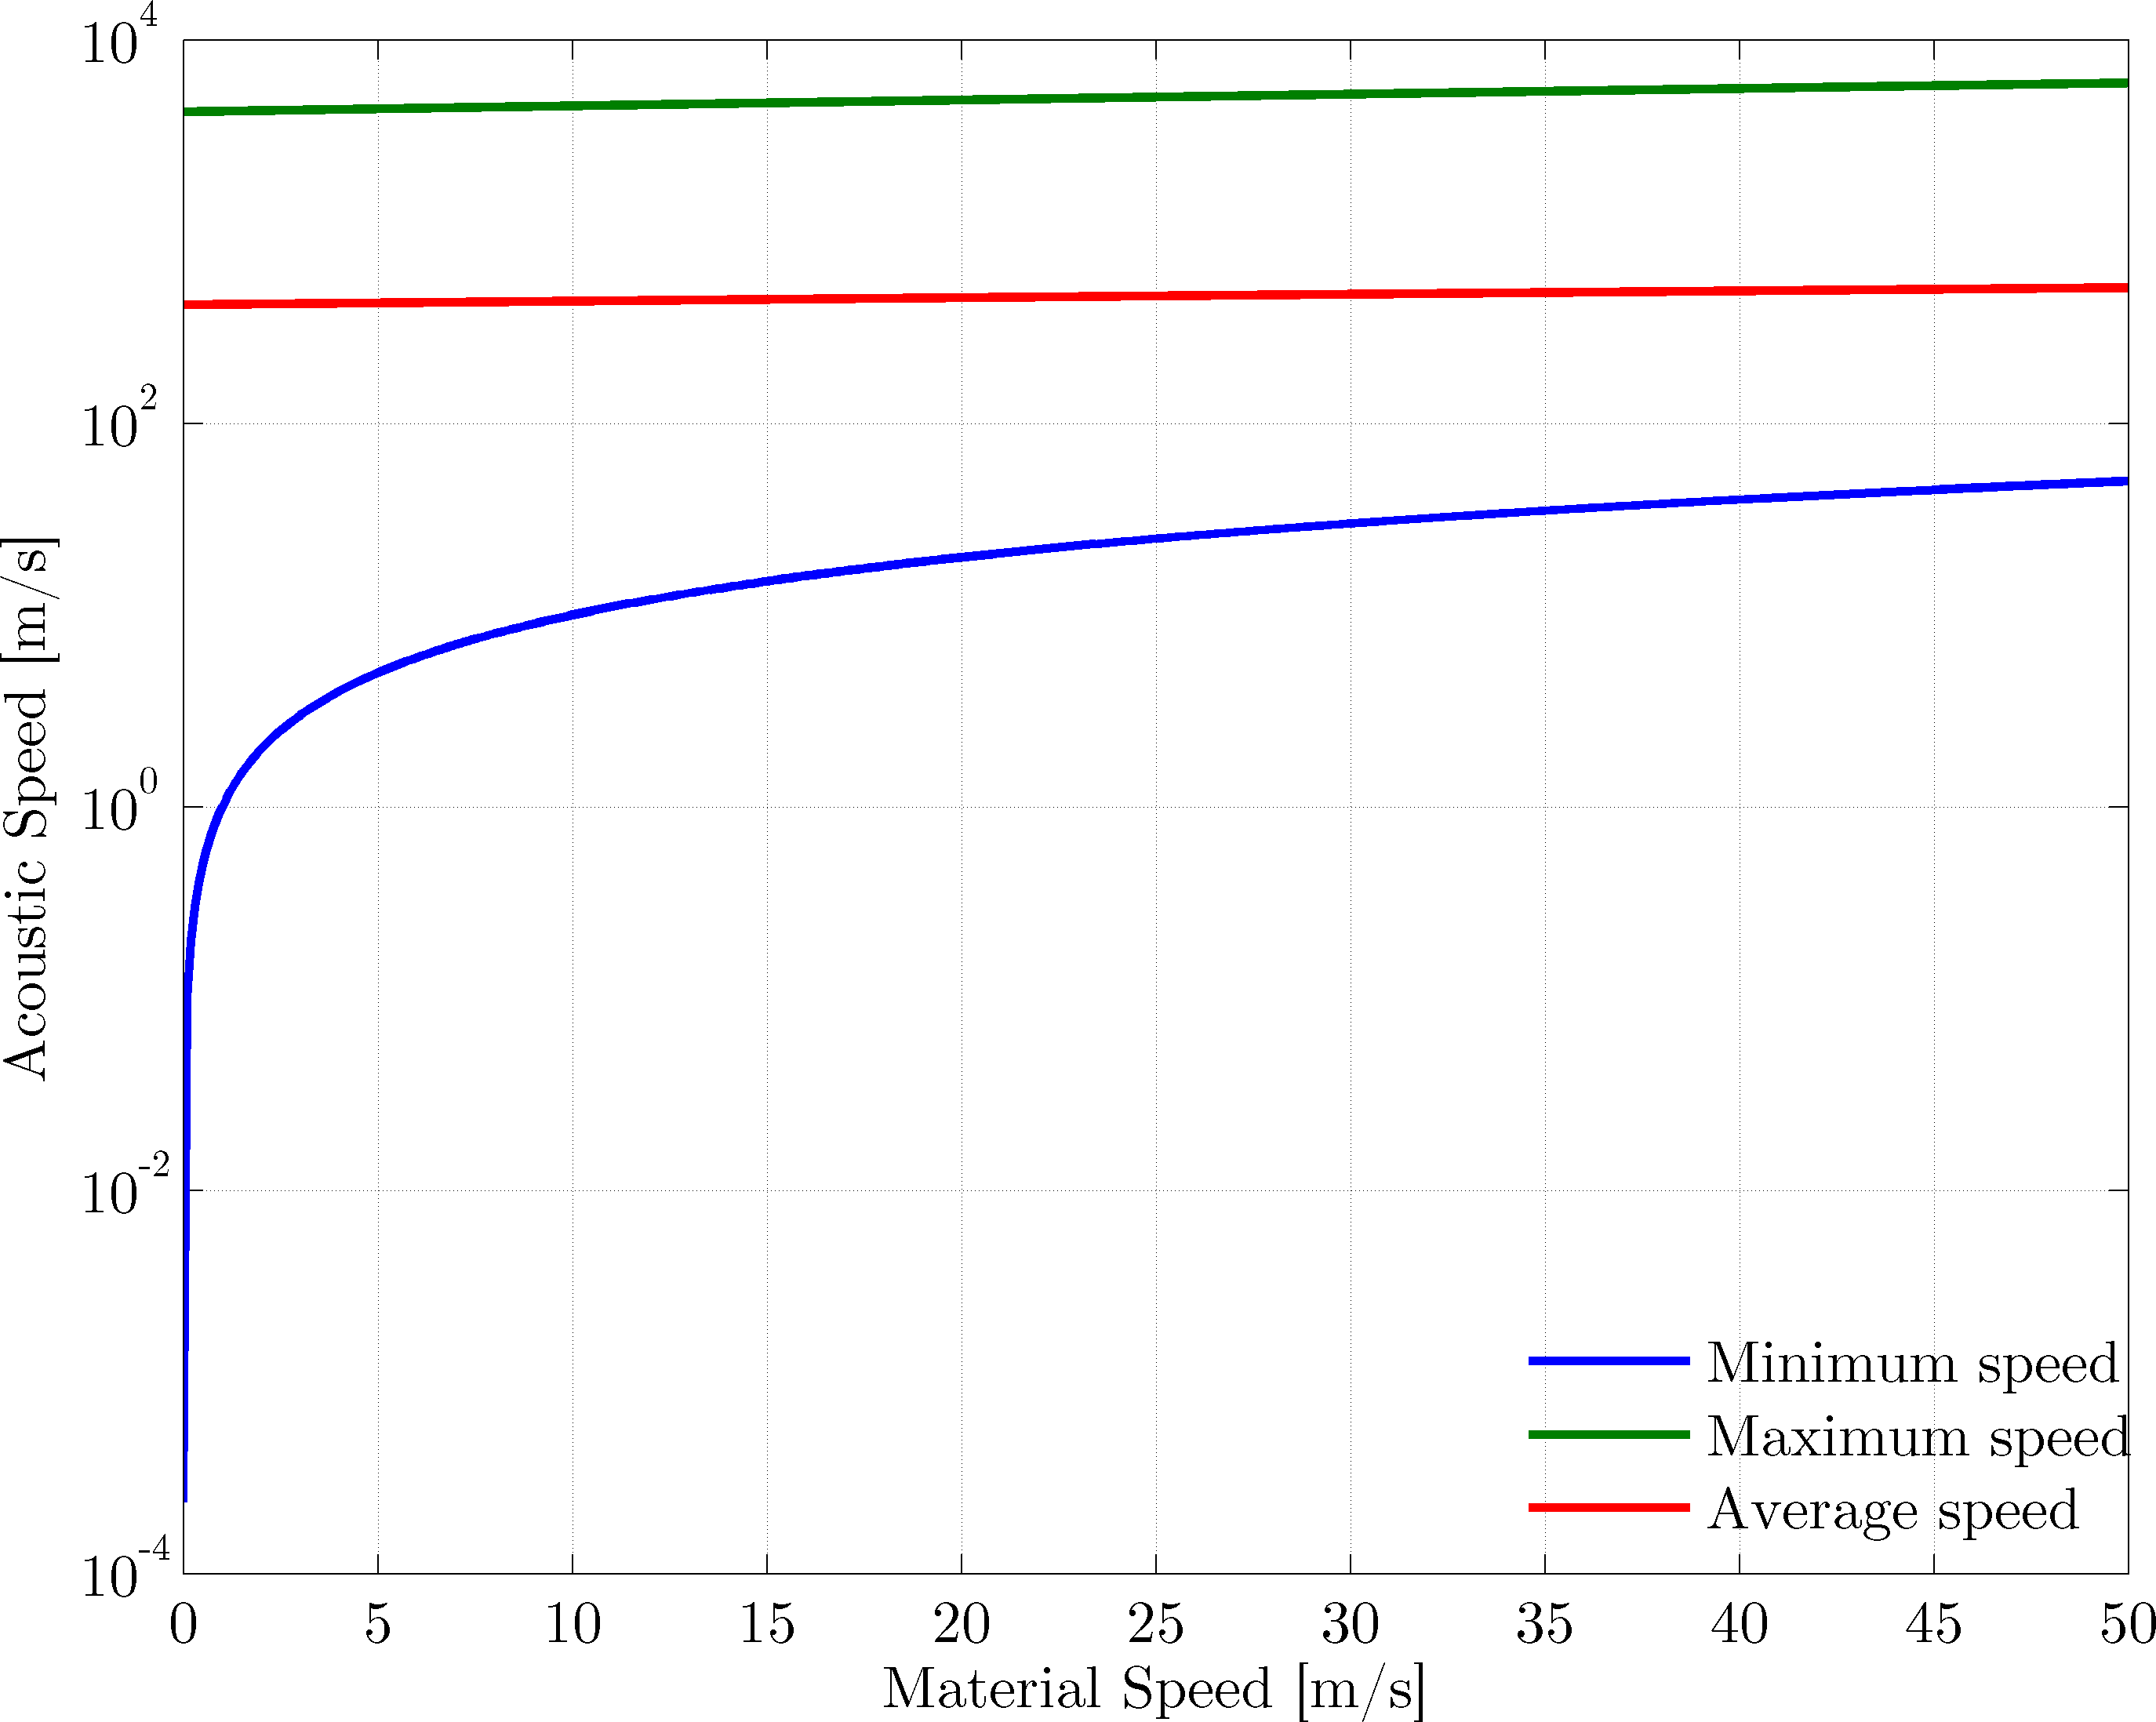
\includegraphics[width=5.0in]{AcousticSpeedVsMaterialSpeed}%
\end{figure}
In order to avoid this, among other reasons \cite{gottlieb_high_2009}, implicit Euler will be explored in this and future work.

